\documentclass{report}
% \documentclass{article}
% Language
\usepackage[T1]{fontenc}
\usepackage[utf8]{inputenc}
\usepackage[english]{babel}


% For commenting
\usepackage{comment}

% Page formatting
\usepackage{geometry}
\geometry{a4paper, margin=25mm, includefoot}

% Font, line height, paragraph indentation
% \usepackage{mathptmx} % Times New Roman
\usepackage{newtxtext, newtxmath} % Times New Roman (Modern + Math symbols)
\linespread{1.2}
\setlength{\parindent}{0pt}
% \usepackage{setspace}

% Chapter/section title formatting
\usepackage{titlesec}
\titleformat{\chapter}[display]{\normalfont\Large}{\chaptertitlename\ \thechapter}{0pt}{\huge\bfseries}[\vspace{8pt}\titlerule]
\titlespacing{\chapter}{0cm}{0cm}{0.5cm}

\titleformat{\paragraph}
{\normalfont\normalsize\bfseries}{\theparagraph}{1em}{}
\titlespacing*{\paragraph}
{0pt}{3.25ex plus 1ex minus .2ex}{1.5ex plus .2ex}

% Multi-column TOC
\usepackage{multicol}
% \makeatletter
% \renewcommand{\tableofcontents}[1][\contentsname]{%
%     \chapter*{#1}
%     \begin{small}
%     % \setlength{\columnseprule}{0.5pt}
%     \setlength{\columnsep}{20pt}
%     \begin{multicols}{2}
%         \@starttoc{toc}
%     \end{multicols}
%     \end{small}
% }
% \makeatother

% Used for moving abstract from the center of the page to the top
\usepackage{etoolbox}
\patchcmd{\abstract}{\null\vfil}{}{}{}

% Figures and captions
% \usepackage{caption}
\usepackage{float}
\usepackage{graphicx}
\usepackage{wrapfig}
\usepackage[font=small,labelfont=bf]{caption}
\usepackage[labelformat=simple]{subcaption}
\renewcommand\thesubfigure{(\alph{subfigure})}

\def \FigureAbbreviaition {Fig.}
\newcommand{\figref}[1]{\FigureAbbreviaition\ \ref{#1}}
\newcommand{\tabref}[1]{Table \ref{#1}}

% Figure caption formatting
\AtBeginDocument{%
\captionsetup[figure]{name={\FigureAbbreviaition},aboveskip=10pt,belowskip=-10pt}
\captionsetup[subfigure]{aboveskip=10pt,belowskip=0pt}
\captionsetup[table]{aboveskip=10pt,belowskip=-10pt}
% \captionsetup[subtable]{aboveskip=10pt,belowskip=0pt}
}

% Array
\usepackage{array}
\usepackage{textpos}

% Math and symbols
% \usepackage{amsmath, amssymb, bm} % newtxmath has same defines as amssymb
\usepackage{amsmath, bm}
\usepackage{mathtools}
\usepackage{verbatim}
\usepackage{xfrac}
\usepackage{tensor}
\usepackage{interval}
\usepackage{commath} % for \abs, \norm
\usepackage{physics} % for qty(), qty{} etc. (automatic parentheses)

% Custom commands
\usepackage{xstring}
\usepackage{xspace}

\newcommand{\fakecite}[0]{\hl{\textbackslash cite}\xspace}
% \renewcommand{\vec}[1]{\ensuremath{\bm{#1}}} % vector [amsmath, bm]
\renewcommand{\vec}[1]{\ensuremath{\bm{\mathrm{#1}}}} % matrix [amsmath, bm]
\newcommand{\mat}[1]{\ensuremath{\bm{\mathrm{#1}}}} % matrix [amsmath, bm]
\newcommand{\T}[0]{\ensuremath{^\mathsf{T}}} % transpose ^T
\newcommand{\inv}[0]{\ensuremath{^{-1}}} % inverse ^{-1}
\newcommand{\pinv}[0]{\ensuremath{^{\dagger}}} % pseudo-inverse ^{-1}
\newcommand{\rvec}[1]{\ensuremath{\renewcommand{\arraystretch}{0.6}\begin{bmatrix} #1 \end{bmatrix}}}
\newcommand{\cvec}[1]{\ensuremath{\renewcommand{\arraystretch}{1.0}\begin{bmatrix} #1 \end{bmatrix}}}
\newcommand{\twodots}{\mathinner {\ldotp \ldotp}} % .. (two dots)
\renewcommand{\secref}[1]{\hyperref[#1]{\ref*{#1}\ \nameref*{#1}}}
% \newcommand{\tf}[3][T]{\ensuremath{\tensor[^{#2}]{\mat{#1}}{_{#3}}}}
\newcommand{\tf}[3][T]{\ensuremath{{\mat{#1}^{#2}_{#3}}}}
\newcommand*\of{\qty} % $f\of(x)$

% usage: \tf{from}{to} | \tf[T]{from}{to} | \tf[R]{from}{to} | \tf[t]{from}{to} etc.
% \newcommand{\tf}[3][T]{%
%     \IfEqCase{#1}{%
%         {T}{\ensuremath{\tensor[^{#2}]{\mat{#1}}{_{#3}}}}%
%         {R}{\ensuremath{\tensor[^{#2}]{\mat{#1}}{_{#3}}}}%
%         {t}{\ensuremath{\tensor[^{#2}]{\vec{#1}}{_{#3}}}}%
%         {p}{\ensuremath{\tensor[^{#2}]{\vec{#1}}{_{#3}}}}%
%     }[\PackageError{tf}{Undefined option: #1}{}]%
% }%

% Equation spacing
\AtBeginDocument{%
\abovedisplayskip=6pt plus 2pt minus 2pt
\abovedisplayshortskip=6pt plus 2pt minus 2pt
\belowdisplayskip=6pt plus 2pt minus 2pt
\belowdisplayshortskip=6pt plus 2pt minus 2pt
}

% SI units + config and custom units
\usepackage{siunitx}[=v2]
\sisetup{
    per-mode=fraction, fraction-function=\sfrac, % fractions
    % round-mode=figures, round-precision=3, % rounding
    output-exponent-marker=\ensuremath{\mathrm{e}},
    separate-uncertainty=true, multi-part-units=single, % for \SI{2 \pm 0.2}{\rad},
    binary-units=true, % for \byte, \giga etc.
}
\DeclareSIUnit \pixel {px}

% Text highlight (\hl)
\usepackage{soul}

% Enumeration and tables
\usepackage{enumerate}
\usepackage{enumitem}
\usepackage{multirow} 
\usepackage{multicol}
\usepackage{ltablex}
\usepackage{spreadtab}
\usepackage{booktabs}
\usepackage{tabto}

\usepackage{diagbox}
\usepackage{tabularx}
\usepackage[export]{adjustbox}

% Custom tables commands for fixed-column sizes
\newcommand{\PreserveBackslash}[1]{\let\temp=\\#1\let\\=\temp}
\newcolumntype{C}[1]{>{\PreserveBackslash\centering}p{#1}}
\newcolumntype{R}[1]{>{\PreserveBackslash\raggedleft}p{#1}}
\newcolumntype{L}[1]{>{\PreserveBackslash\raggedright}p{#1}}

% Enumeration formatting
\newcommand{\tabitem}{~~\llap{\textbullet}~~}
\newcommand{\sqrbulletsml}{\textcolor{black}{\raisebox{.45ex}{\rule{.6ex}{.6ex}}}}
\newcommand{\sqrbulletmed}{\textcolor{black}{\raisebox{.40ex}{\rule{.7ex}{.7ex}}}}

\renewcommand{\labelitemi}{\sqrbulletmed}
\renewcommand{\labelitemii}{\sqrbulletsml}
\renewcommand{\labelitemiii}{\sqrbulletsml}
\renewcommand{\labelitemiv}{\sqrbulletsml}

% Colors (latexcolor.com)
\usepackage{xcolor}
\definecolor{cerulean}{rgb}{0.0, 0.48, 0.65}
\definecolor{earthyellow}{rgb}{0.88, 0.66, 0.37}
\definecolor{darkmagenta}{rgb}{0.55, 0.0, 0.55}
\definecolor{darkolivegreen}{rgb}{0.33, 0.42, 0.18}
\definecolor{codegray}{gray}{0.9}
\definecolor{gainsboro}{rgb}{0.86, 0.86, 0.86}
\definecolor{cyan}{rgb}{0.0, 1.0, 1.0}

\definecolor{light-yellow}{RGB}{255, 255, 137}
\definecolor{light-blue}{RGB}{148, 201, 233}

% colored square box
% https://tex.stackexchange.com/questions/201300/inline-boxes-alternative-to-pifonts-non-filled-but-shadowed-box
\newcommand{\sqbox}[1]{\textcolor{#1}{\rule{1.2ex}{1.2ex}}}

% Code snippets
\usepackage{listings}
% \renewcommand{\arraystretch}{1.2}
\renewcommand{\tabcolsep}{0.2cm}

% Code snippets formatting
\lstset{
    backgroundcolor=\color{black!5},        % set backgroundcolor
    basicstyle=\footnotesize\ttfamily,      % basic font setting
    captionpos=b,                           % caption position
    frame=single,                           % draw a frame at the top and bottom of the code block
    framesep=5pt,                           % frame margin
    xleftmargin=5pt,                        % frame margin
    xrightmargin=5pt,                       % frame margin
    tabsize=4,                              % tab space width
    showstringspaces=false,                 % don't mark spaces in strings
    breaklines=true,                        % wrap lines
    commentstyle=\color{darkolivegreen},    % comment color
    keywordstyle=\color{darkmagenta},       % keyword color
    stringstyle=\color{earthyellow},        % string color
    identifierstyle=\color{cerulean},
}

% Custom inline-code command (\code)
%\newcommand{\lstinln}[1]{\colorbox{gainsboro}{\texttt{#1}}}
\newcommand{\code}[1]{%
  \begingroup\setlength{\fboxsep}{2pt}%
  \colorbox{gainsboro}{\texttt{\hspace{2pt}\vphantom{Ay}#1\hspace{2pt}}}%
  \endgroup
}

% Appendices
\usepackage[toc]{appendix}

% Bibliography and citation
\usepackage[style=numeric, sorting=none]{biblatex}
\usepackage{csquotes}
\DeclareNameAlias{sortname}{family-given}
\DeclareNameAlias{default}{family-given}

\addbibresource{resources.bib}

% Section cross-referencing
\usepackage{nameref}
\usepackage{hyperref}

% Label counter formatting (e.g. Figure 1 or Figure 2.1)
% used for continuous numbering (1, 2, 3 ..) through all chapters
\usepackage{chngcntr} 
\AtBeginDocument{%
    \counterwithout{figure}{section}
    \counterwithout{table}{section}
    \counterwithout{equation}{section}
    \counterwithout{lstlisting}{section}
}

% Glossaries and acronyms
% must be loaded last + no empty includes in main document.
\usepackage[automake, acronym, nogroupskip, nonumberlist]{glossaries}
\usepackage{glossary-mcols}
\setglossarysection{section}

% command for dual entries
% \newdualentry[<options>]{<label>}{<abbrv>}{<long>}{<description>}
% https://tex.stackexchange.com/a/368666
\newcommand*{\newdualentry}[5][]{%
  \newglossaryentry{main-#2}{%
    name={#4 (\glslink{#2}{#3})},%
    text={#3\glsadd{#2}},%
    description={{#5}},%
    #1%
  }%
  \newglossaryentry{#2}{%
    type=\acronymtype,%
    first={\glslink{main-#2}{#4 (#3)}},%
    name={#3\glsadd{main-#2}},%
    description={\glslink{main-#2}{#4}},%
    plural={#2s},%
    firstplural={\glsentrydesc{#2}s (\glsentryplural{#2})}
  }%
}

% setup and load glossaries
\makeglossaries
\loadglsentries{glossary}

% only hyperlink first-time glossary entries
% \renewcommand*{\glslinkcheckfirsthyperhook}{%
%   \ifglsused{\glslabel}%
%   {%
%     \setkeys{glslink}{hyper=false}%
%   }%
%   {}%
% }

% generate word count text file wc.tex
\immediate\write18{bash wc.sh}

\begin{document}

% title page

\begin{titlepage}
    \begin{center}
   
        {\LARGE Deep reinforcement learning for the board game Dominion\par}


        \vspace{1cm}
        \textbf{An assignment for the course AI tools}
        \vspace{0.5cm}
       
        written by
       
        \vspace{0.5cm}
        
        \begin{tabular}[t]{c@{\extracolsep{4em}}}
        \textbf{Peter Khiem Duc Tinh Nguyen}\\
        Pengu20@student.sdu.dk\\
        \end{tabular}

        \vspace{1.0cm}
        \textbf{Course lector:} Xiaofeng Xiong\\
        \textbf{ECTS:} 5\\
        
\includegraphics[width = 10cm]{img/SDU_logo.jpg}

        \vspace{2cm}

        The code for this project is available at\\
        \textcolor{red}{when the code is public put the github link in the curly brackets}
        \url{https://gitlab.sdu.dk/sdurobotics/medical/student-projects/2023/Peter_Duc_Bachelor_NLP}

        \vfill
        
        \textbf{the Faculty of Engineering (TEK)}\\  
        University of Southern Denmark 
       

        \vspace{0.5cm}
        
        Date of Hand In
        31. of May
    \end{center}
            
\end{titlepage}


% preface
% \input{sections/0-preface}

% roman numbering for abstract, TOC, glossary etc.
\pagenumbering{roman}

% abstract
\clearpage
\begin{abstract}
\setlength{\parindent}{0pt}
\normalsize
The aim of this thesis is to create a system capable of controlling the motion of a 6-DOF manipulator, equipped with a parallel gripper, using natural language. The manipulator is a UR5e robot arm, and the parallel gripper is a Hand-e robotiq gripper. The intent is to enable an arbitrary user to solve tasks using the robot, without the user needing prior knowledge about robot control.
\\\\
The system is created using three pipelines. The first pipeline processes natural language and outputs grammatical information. The second pipeline parses the information into executable actions for the robot. The third pipeline executes the actions on the robot. Furthermore, the system can also calculate and store positions and frames in space. These points and frames are used to set up tasks in the robot manipulator's work environment.
\\\\
The system is evaluated based on a test using volunteers that solves robot manipulation tasks using natural language. The results show that the system has a 70\% success rate in interpretation, in which 50\% of all errors stems from the users formulating instructions for moving the robot relatively. The reason is that they typically use context-based language that the system cannot interpret. An example is \textit{'move up to the height of the starting position of the task'}, where an interpretable alternative is \textit{'move 20 centimeters along the z-axis'}.
\\\\
The final conclusion is that the system performs with 70\% success rate, but does not support the use of context-based language along with high level instructions that contain several actions, like \textit{'remove all blocks from the table'}. Based on user experience, these abilities would likely increase the success rate of the system.
\end{abstract}

% table of contents
\clearpage
\tableofcontents

% workload distribution
\clearpage

\section*{Acknowledgements}
My acknowledgements


\addcontentsline{toc}{section}{Acknowledgments}

% glossary & acronyms
\clearpage
\addcontentsline{toc}{section}{Acronyms and Terms}
\printglossary[type=acronym, title=Acronyms, style=mcolindex]
\printglossary[type=main, title=Terms]

% main document
\clearpage
\pagenumbering{arabic}
\glsresetall

\pagebreak
\chapter{Example section}\label{ch:example}

This document demonstrate the use of figures, references, SI units, glossary, math notation, lists, and otherwise relevant formatting specifications. Paragraphs are typically separated using \texttt{\textbackslash medskip}.\medskip

\begin{figure}[H]
    \centering
    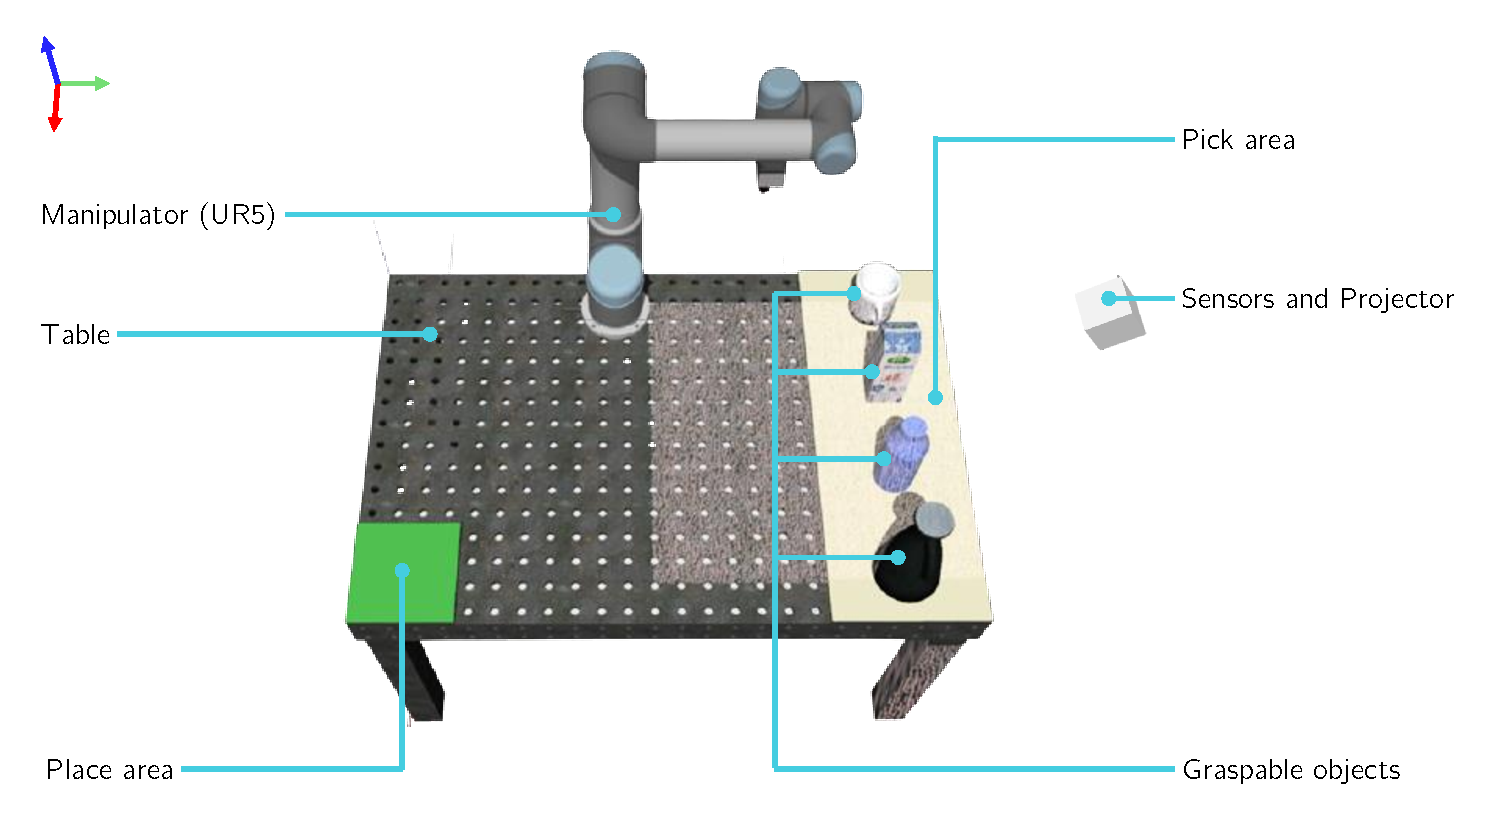
\includegraphics[width=.6\linewidth]{chapters/example/fig/figure.pdf}
    \caption{An example image using \acrlong{acronym-label}.}
    \label{fig:example-figure}
\end{figure}

To exemplify math notation, consider the mapping between the joint configuration of a robot
%
\begin{equation}
    \vec{q} = \rvec{q_1 & q_2 & \dots & q_n}\T,
    \label{eq:jnt-config}
\end{equation}

and \gls{glossary-label}, given as a homogeneous transformation
%
\begin{equation}
    \renewcommand{\arraystretch}{1.2}
    \tf{A}{B} = \begin{bmatrix}
        \tf[R]{A}{B}         & \tf[t]{A}{B} \\
        \vec{0}^{1 \times 3} & 1 
    \end{bmatrix},
\end{equation}

where \tf[R]{A}{B} and \tf[t]{A}{B} is the rotation and translation, respectively, from frame $\{A\}$ to frame $\{B\}$, denoted using a homogeneous transformation matrix $\mat{T}(\vec{q}) \in \mathbb{R}^{4 \times 4}$ as a function of the joint configuration in \eqref{eq:jnt-config}, as described in \cite{robotics-book}.\medskip

Complex table/figure hybrids with aligned captions and functioning labels can be implemented using \texttt{minipage}, as shown in \tabref{tab:example-table} and \figref{fig:example-plot}. Use \fakecite as a placeholder for citations.

\begin{center}
    \renewcommand{\arraystretch}{1.2}
    \begin{minipage}{.4\linewidth}
        \vspace{-10pt}
        \centering
        \begin{tabular}{|l|c|c|c|}
        \hline
        \diagbox[width=5.5em, font=\footnotesize\bfseries]{Method}{Pose} & 1 & 2 & 3 \\ \hline
        Linear    & \SI{18.97}{\second} & \SI{20.35}{\second} & \SI{22.85}{\second} \\ \hline
        Parabolic & \SI{13.66}{\second} & \SI{14.93}{\second} & \SI{17.33}{\second} \\ \hline
        \end{tabular}%
    \end{minipage}%
    \hfill%
    \begin{minipage}{.55\linewidth}
        \vspace{0pt}
        \centering
        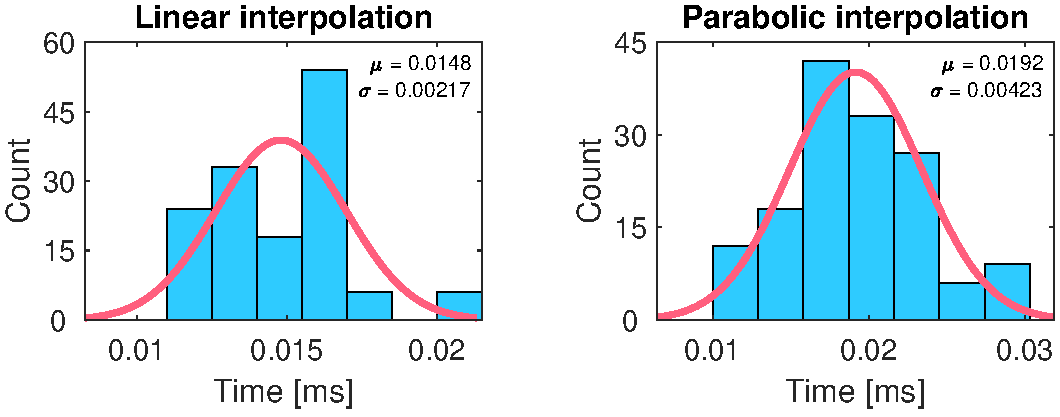
\includegraphics[width=.95\textwidth]{chapters/example/fig/plot.pdf}
    \end{minipage}%
    %    
    \vspace{15pt}
    %
    \begin{minipage}[t]{.4\linewidth}
        \vspace{0pt}
        \captionsetup{type=table}
        \captionof{table}{Trajectory durations of the interpolation-based trajectory generation methods.}
        \label{tab:example-table}
    \end{minipage}%
    \hfill%
    \begin{minipage}[t]{.55\linewidth}
        \vspace{0pt}
        \captionsetup{type=figure}
        \captionof{figure}{Average planning time for each of the interpolation-based trajectory generation methods.}
        \label{fig:example-plot}
    \end{minipage}%
\end{center}

For numbers, units and ranges, the \texttt{siunitx} package is used, which allows to express a number \num{10}, a range of \SIrange{5}{6}{\second}, or a SI unit of \SI{5.73 \pm 1.09}{\second}. Inline row-vectors (with the transpose symbol) can be written as $\vec{a} = \rvec{\vec{a}_p & \vec{a}_o}\T$, where as parentheses can be automatically written using $\qty(a, b)$ or $\qty{\frac{a}{b}, c}$. Also, shorthands for \mat{A}\inv, \mat{A}\pinv and \mat{A}\T.\medskip

\glsresetall

\pagebreak
\chapter{Introduction} \label{ch:intro}

Subject matter terms are addressed with \texttt{\textbackslash gls\{glossary-label\}} like so \gls{glossary-label}. \\
Acronyms are addressed with either with their long equivalent \texttt{\textbackslash acrlong\{gls-label\}} which gives \acrlong{acronym-label}
or the short equivalent \texttt{\textbackslash acrshort\{gls-label\}} which gives \acrshort{acronym-label}. \\
Subject matter terms can also be multi structure \texttt{\textbackslash gls\{glossary-multi-label\}} which gives \gls{glossary-multi-label}
(see terms and acronyms above).


\pagebreak
\chapter{Problem 1} \label{ch:problem1}


\section{Introduction} \label{sec:problem1-introduction}
Here we write the introduction for problem 1.


\section{Related Work} \label{sec:problem1-related-work}

Here we cite the related work by \texttt{\textbackslash cite\{source-label\}} like this \cite{example-article}

\pagebreak
\chapter{Problem 2} \label{ch:problem2}

\pagebreak
\chapter{Discussion} \label{ch:discussion}

\pagebreak
\chapter{Conclusion} \label{ch:conclusion}


% bibliography
\pagebreak
% \printbibliography[heading=bibintoc]
\begin{multicols}{2}[\printbibheading]
\printbibliography[heading=none]
\end{multicols}

\appendix
\chapter{Appendix A Title}

\end{document}